%\documentclass[dvipdfmx]{beamer}      % platex の場合
\documentclass[handout]{beamer}        % lualatex の場合
\usepackage{mySld}
\usepackage{multicol}

\begin{document}
\title{基礎コンピュータ工学\\第5章 機械語プログラミング\\(パート1)}
\date{}

\begin{frame}
  \titlepage
  \centerline{\url{https://github.com/tctsigemura/TecTextBook}}
  \vfill
  \centerline{本スライドの入手:
    \raisebox{-7mm}{
\includegraphics[scale=0.3]{../Img/QRs5_1.png}}}
\end{frame}

%==============================================================================
%\begin{frame}
%  \frametitle
%  \tableofcontents
%\end{frame}

\section{機械語プログラミング}
%==============================================================================
\begin{frame}
  \frametitle{本科目の目的を再確認}
  \emph{「ノイマン型コンピュータ」の基本原理を学ぶ.}\\
  (99%以上のコンピュータはノイマン型だから.)
  \vfill
  これまでに学んだこと.
  \begin{enumerate}
    \item[(1)] 情報の表現(2進数(ON/OFF)で情報を表現できる.)\\
      おおかみ情報,数値(計算,負数,小数),文字
      \vfill
    \item[(2)] コンピュータの基本回路(2進数の計算や記憶ができる.)\\
      NOT,AND,OR,XOR,加算器,RS-FF
      \vfill
    \item[(3)] マイコンの組み立てと操作\\
      ハンダ,コンソールパネル,レジスタ,フラグ,メモリ
  \end{enumerate}
  \vfill
\end{frame}

%==============================================================================
\begin{frame}
  \frametitle{コンピュータとは}
  \begin{itemize}
  \item コンピュータって何?\\
    Compute(計算する) + er(もの) = Computer(計算機)\\
    もともとは,数値計算をするための機械
    \vfill
  \item 計算機?(電卓と何が違うの?) \\
    計算手順を記憶することができる.(平均点を計算する例)\\
    \vfill
    電卓:
    \vfill
    コンピュータ:
    \vfill
    \emph{ノイマン型コンピュータは計算手順を記憶できる.}
  \end{itemize}
\end{frame}

%==============================================================================
\begin{frame}
  \frametitle{ノイマン型コンピュータの特徴}
  \begin{itemize}
  \item \emph{プログラム内蔵方式(ストアード・プログラム方式)} \\
    データだけでなく,プログラムもメモリに記憶する.
    \vfill
  \item \emph{逐次実行方式} \\
    メモリに記憶したプログラムの命令を,\\
    一つ一つ順番に(自動的に)実行する.
    \vfill
  \item \emph{2進法} \\
    コンピュータ内部の情報表現は,\\
    ハードウェアで扱いやすい2進数を用いる.
    \vfill
  \end{itemize}
\end{frame}

%==============================================================================
\begin{frame}
  \frametitle{コンピュータの構成(一般的)}
  \begin{minipage}{0.59\columnwidth}
    \centerline{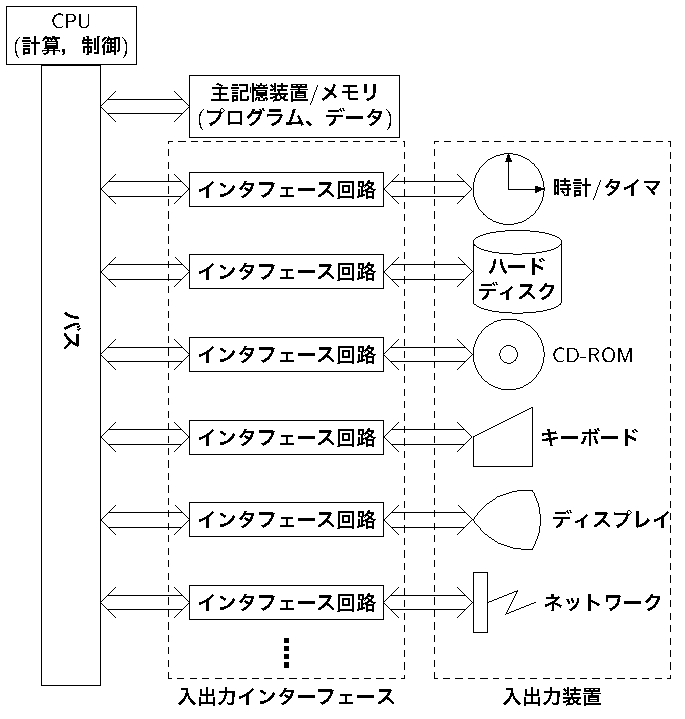
\includegraphics[scale=0.63]{../Tikz/kousei1.pdf}}
  \end{minipage}
  \begin{minipage}{0.4\columnwidth}
    \begin{itemize}
    \item CPU\\
      {\small(Central Processing Unit)}\\
      {\small(中央処理装置)}\\
      \vspace{4ex}
    \item 主記憶装置(メモリ)\\
      \vspace{4ex}
    \item 入出力インターフェース\\
      \vspace{4ex}
    \item 入出力装置\\
      \vspace{4ex}
    \item バス(BUS)\\
      \vspace{6ex}
    \end{itemize}
  \end{minipage}
\end{frame}

%==============================================================================
\begin{frame}
  \frametitle{コンピュータの構成(TeCの場合)}
  \begin{minipage}{0.59\columnwidth}
    \centerline{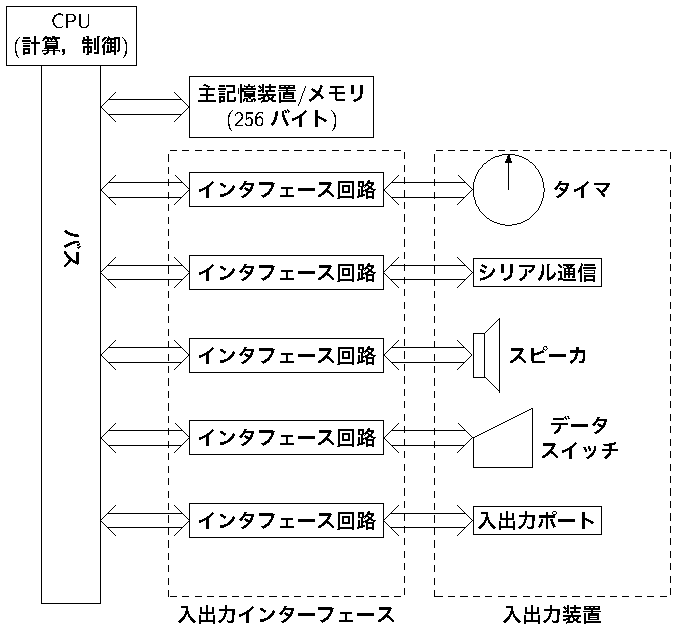
\includegraphics[scale=0.63]{../Tikz/kousei2.pdf}}
  \end{minipage}
  \begin{minipage}{0.4\columnwidth}
    \begin{itemize}
    \item CPU\\
      \vspace{5ex}
    \item 主記憶装置(メモリ)\\
      \vspace{5ex}
    \item 入出力インターフェース\\
      \vspace{4ex}
    \item 入出力装置\\
      \vspace{4ex}
    \item バス(BUS)\\
      \vspace{6ex}
    \end{itemize}
  \end{minipage}
\end{frame}

%==============================================================================
\begin{frame}
  \frametitle{TeC内部の記憶装置}
  \vfill
  \centerline{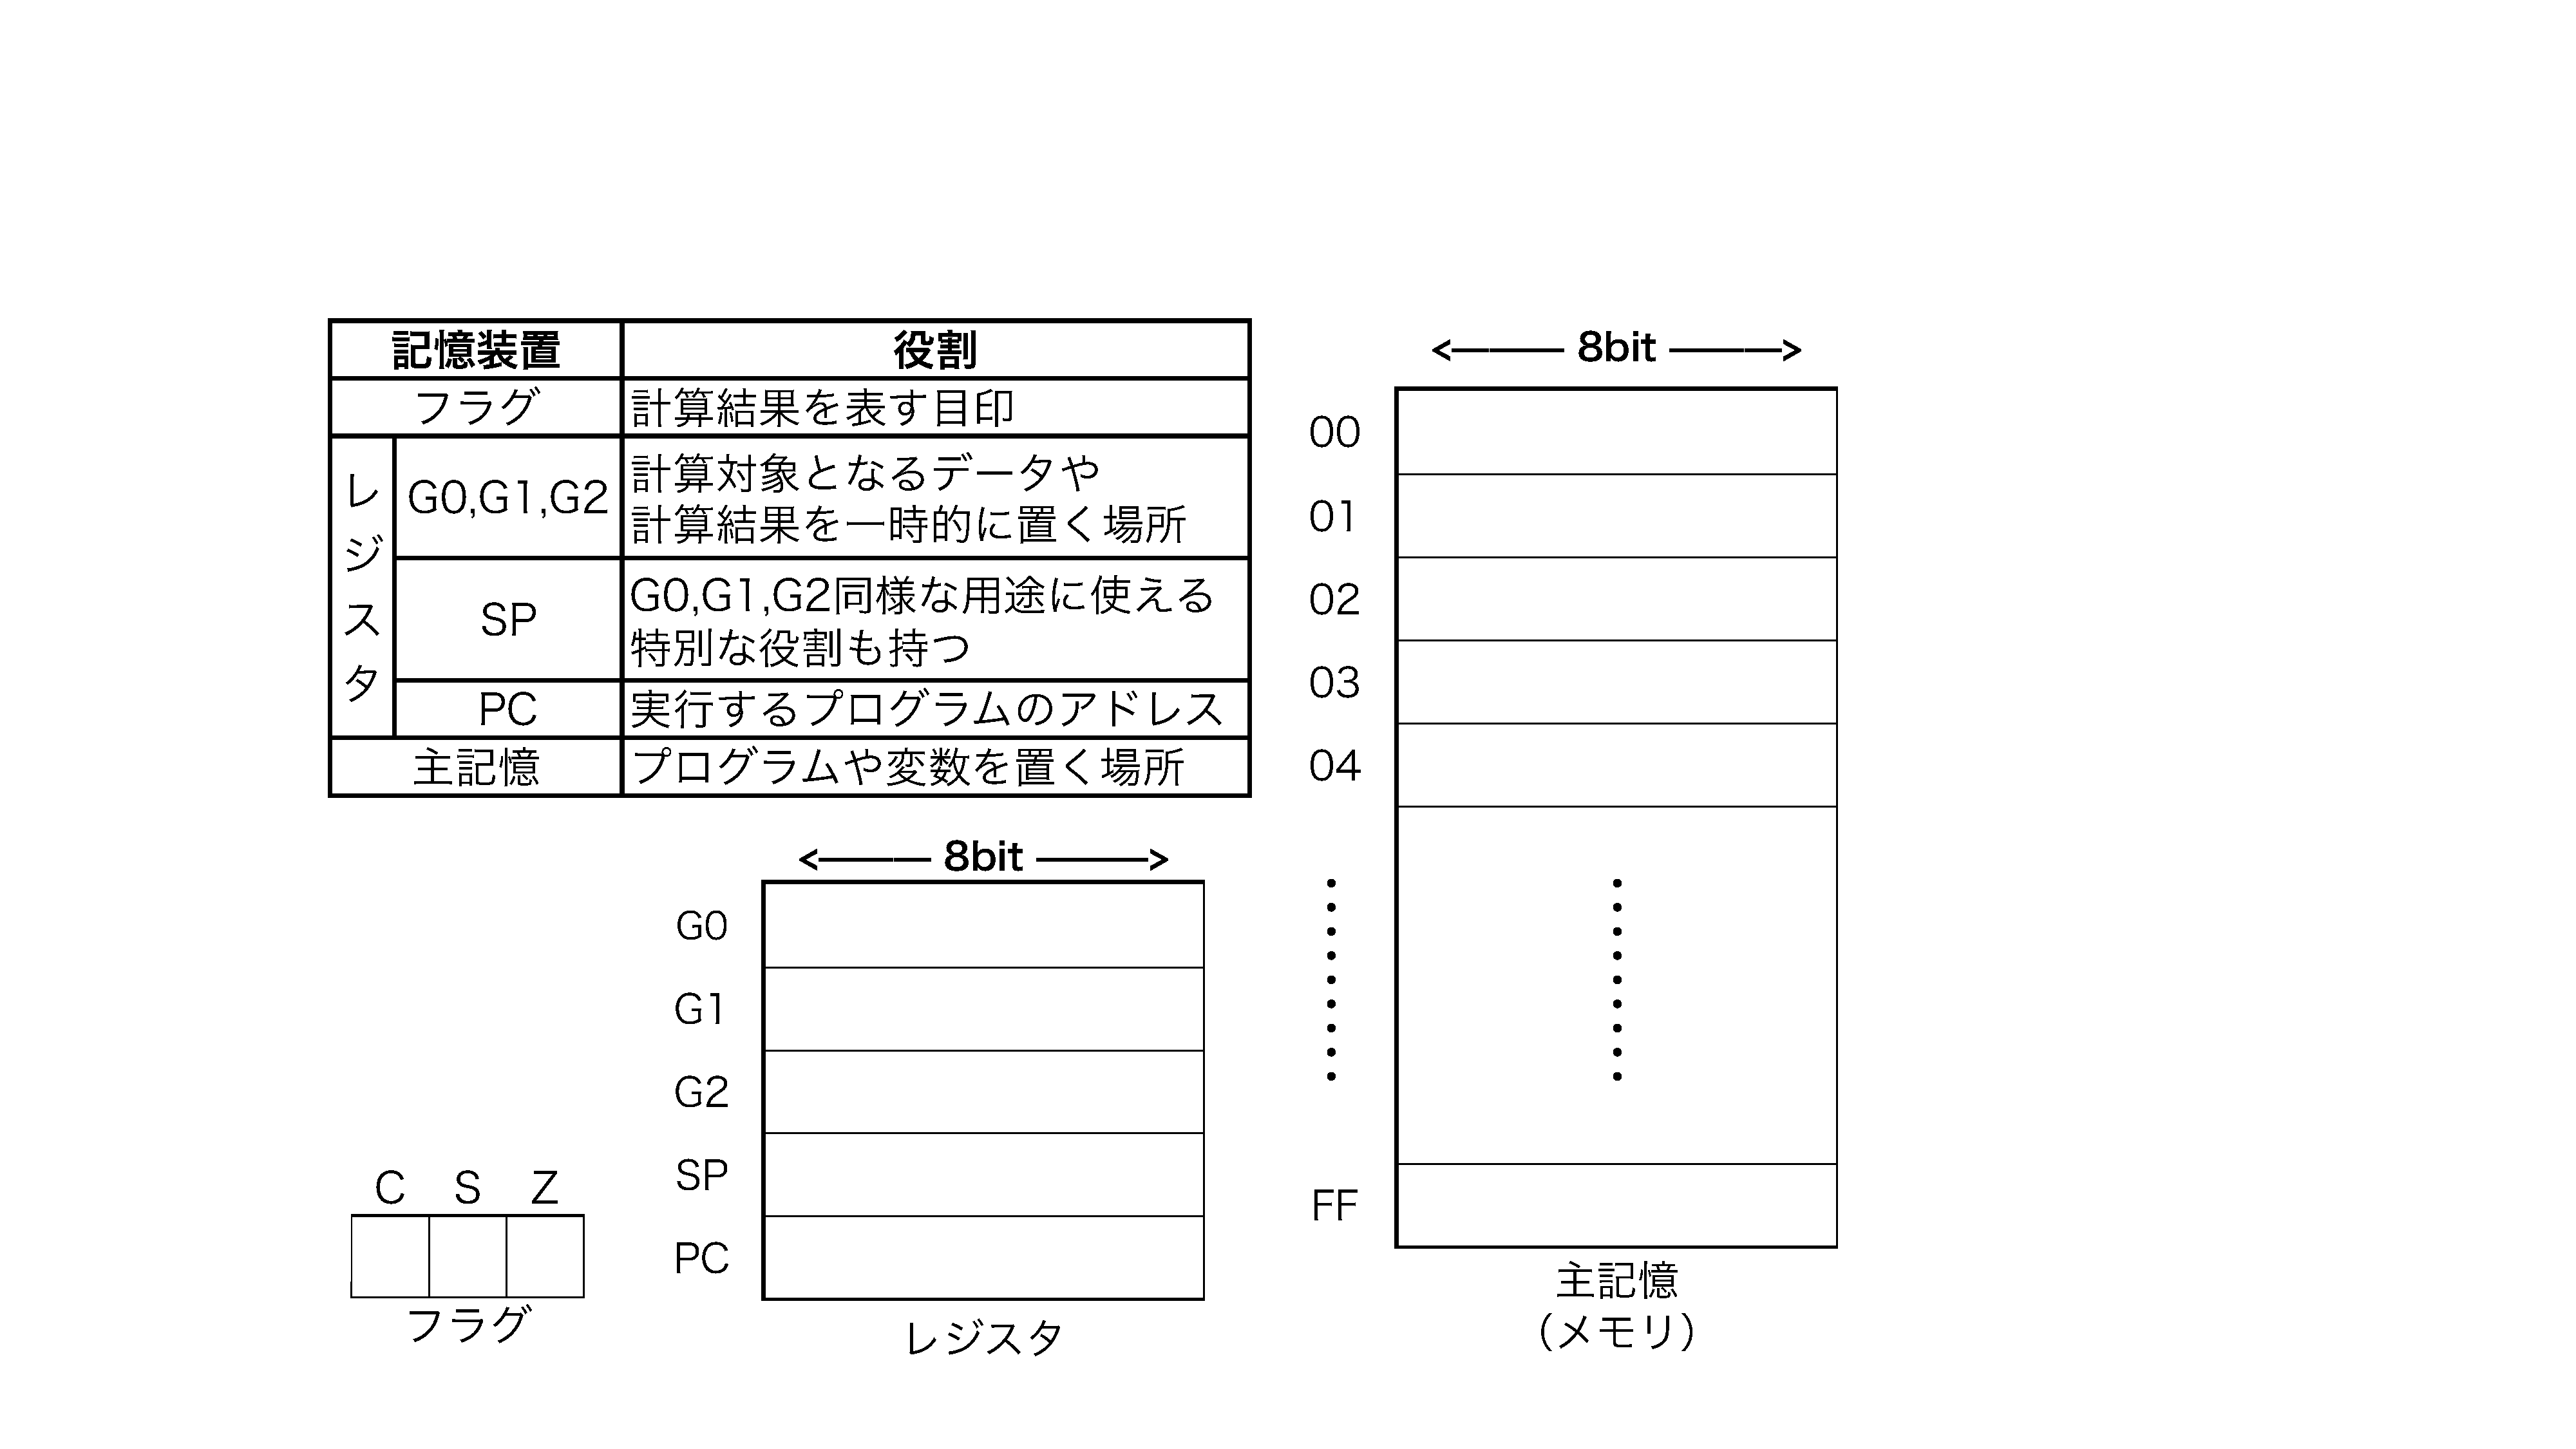
\includegraphics[scale=0.7]{../chap4/naibu.pdf}}
  \vfill
  \begin{itemize}
    \item フラグ
    \item レジスタ:PC(Program Counter)は\emph{逐次実行}の要
    \item 主記憶:プログラムとデータを置く(\emph{ストアード・プログラム方式})
  \end{itemize}
  \vfill
\end{frame}

%==============================================================================
\begin{frame}
  \frametitle{機械語プログラミングと機械語命令}
  \emph{「機械語(Machine Language)」}=機械(CPU)の言語\\
  \vfill
  \vfill
  \emph{「機械語プログラミング」}=機械語プログラムを作る作業のこと\\
  \vfill
  \emph{「機械語プログラム」}=機械語命令で記述したプログラムのこと\\
  \vfill
  \emph{「機械語命令」}=機械(CPU)が理解できる命令のこと\\
  (機械語命令は2進数で表現する.)
  \vfill
  \emph{機械語プログラムの例}\\
       {\ttfamily\small\begin{center}
         \begin{tabular}{|c|c|c|} \hline
           機械語命令 & ニーモニック & 意味\\
           \hline
           $0000~0000_{2}$ & NO & No Operation \\
           $1111~1111_{2}$ & HALT & Halt \\
           \hline
         \end{tabular}\\
       \emph{「ニーモニック」}=命令の意味の英語を簡略化した綴
       \end{center}}
\end{frame}

%==============================================================================
\begin{frame}
  \frametitle{機械語命令の実行}
  \vfill
  \centerline{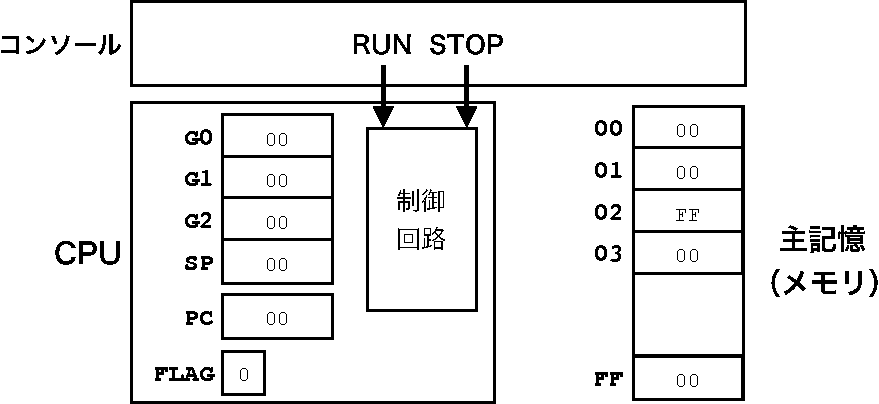
\includegraphics[scale=0.7]{exec-crop.pdf}}
  \vfill
  CPUは以下を繰り返し機械語プログラムを実行する.
  \begin{enumerate}
  \item[1.] CPUはメモリからプログラムの\emph{機械語命令}を一つ取出す.
  \item[2.] CPUは機械語命令の種類を調べる.
  \item[3.] CPUは機械語命令の内容により計算などを行う.
  \item[4.] CPUは次の機械語命令について1.〜3.を行う.
  \end{enumerate}
  \vfill
\end{frame}

%==============================================================================
\begin{frame}
  \frametitle{演習}
  \emph{逐次実行とPC(Program Counter)の働きを確認する.}\\
  以下のプログラムを実行した後のPCの値はいくつになるか?\\
  \begin{multicols}{3}
  {\ttfamily\small\begin{center}
    \begin{tabular}{c|c|l}
      \multicolumn{1}{c}{番地} & \multicolumn{1}{c}{命令} &  \\
      \cline{2-2}
      $00_{16}$ & $00_{16}$ & NO \\
      $01_{16}$ & $FF_{16}$ & HALT \\
      \cline{2-2}
    \end{tabular}
    \columnbreak
    \begin{tabular}{c|c|l}
      \multicolumn{1}{c}{番地} & \multicolumn{1}{c}{命令} &  \\
      \cline{2-2}
      $00_{16}$ & $00_{16}$ & NO \\
      $01_{16}$ & $00_{16}$ & NO \\
      $02_{16}$ & $00_{16}$ & NO \\
      $03_{16}$ & $FF_{16}$ & HALT \\
      \cline{2-2}
    \end{tabular}
%    \columnbreak
    \begin{tabular}{c|c|l}
      \multicolumn{1}{c}{番地} & \multicolumn{1}{c}{命令} &  \\
      \cline{2-2}
      $00_{16}$ & $00_{16}$ & NO \\
      $01_{16}$ & $00_{16}$ & NO \\
      $02_{16}$ & $00_{16}$ & NO \\
      $03_{16}$ & $00_{16}$ & NO \\
      $04_{16}$ & $00_{16}$ & NO \\
      $05_{16}$ & $00_{16}$ & NO \\
      $06_{16}$ & $FF_{16}$ & HALT \\
      \cline{2-2}
    \end{tabular}
  \end{center}}
  \end{multicols}
  \vfill
  \emph{次の言葉の意味を確認しなさい.}
  \begin{multicols}{2}
  \begin{itemize}
  \item プログラム内蔵方式
  \item 逐次実行方式
  \item 2進法
  \item CPU,メモリ
  \item PC
  \item 機械語
  \item ニーモニック
  \item NO,HALT
  \end{itemize}
  \end{multicols}
  \vfill
\end{frame}

%==============================================================================
%\begin{frame}
%  \frametitle{}
%\end{frame}

\end{document}
